

\tikzset{every picture/.style={line width=0.75pt}} %set default line width to 0.75pt        

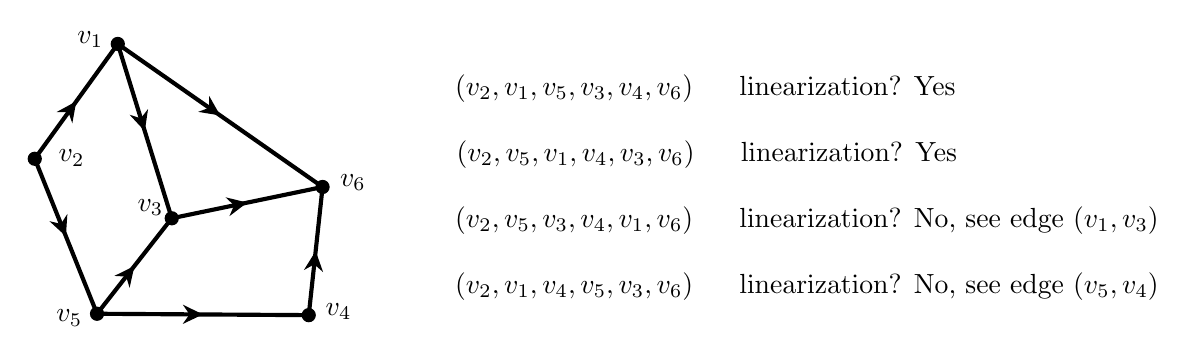
\begin{tikzpicture}[x=0.5pt,y=0.5pt,yscale=-1,xscale=1]
%uncomment if require: \path (0,228); %set diagram left start at 0, and has height of 228

%Flowchart: Connector [id:dp3072392280017706] 
\draw  [fill={rgb, 255:red, 0; green, 0; blue, 0 }  ,fill opacity=1 ] (78,14) .. controls (78,11.58) and (79.96,9.62) .. (82.38,9.62) .. controls (84.79,9.62) and (86.75,11.58) .. (86.75,14) .. controls (86.75,16.42) and (84.79,18.38) .. (82.38,18.38) .. controls (79.96,18.38) and (78,16.42) .. (78,14) -- cycle ;
%Flowchart: Connector [id:dp21397717392367266] 
\draw  [fill={rgb, 255:red, 0; green, 0; blue, 0 }  ,fill opacity=1 ] (63,209) .. controls (63,206.58) and (64.96,204.62) .. (67.38,204.62) .. controls (69.79,204.62) and (71.75,206.58) .. (71.75,209) .. controls (71.75,211.42) and (69.79,213.38) .. (67.38,213.38) .. controls (64.96,213.38) and (63,211.42) .. (63,209) -- cycle ;
%Flowchart: Connector [id:dp8067973087407497] 
\draw  [fill={rgb, 255:red, 0; green, 0; blue, 0 }  ,fill opacity=1 ] (18,97) .. controls (18,94.58) and (19.96,92.62) .. (22.38,92.62) .. controls (24.79,92.62) and (26.75,94.58) .. (26.75,97) .. controls (26.75,99.42) and (24.79,101.38) .. (22.38,101.38) .. controls (19.96,101.38) and (18,99.42) .. (18,97) -- cycle ;
%Flowchart: Connector [id:dp962987276172525] 
\draw  [fill={rgb, 255:red, 0; green, 0; blue, 0 }  ,fill opacity=1 ] (117,140) .. controls (117,137.58) and (118.96,135.62) .. (121.38,135.62) .. controls (123.79,135.62) and (125.75,137.58) .. (125.75,140) .. controls (125.75,142.42) and (123.79,144.38) .. (121.38,144.38) .. controls (118.96,144.38) and (117,142.42) .. (117,140) -- cycle ;
%Straight Lines [id:da5158988833498211] 
\draw [color={rgb, 255:red, 0; green, 0; blue, 0 }  ,draw opacity=1 ][line width=1.5]    (22.38,97) -- (82.38,14) ;
\draw [shift={(52.38,55.5)}, rotate = 125.86] [fill={rgb, 255:red, 0; green, 0; blue, 0 }  ,fill opacity=1 ][line width=0.08]  [draw opacity=0] (14.56,-6.99) -- (0,0) -- (14.56,6.99) -- (9.67,0) -- cycle    ;
%Straight Lines [id:da26521146489140124] 
\draw [color={rgb, 255:red, 0; green, 0; blue, 0 }  ,draw opacity=1 ][line width=1.5]    (67.38,209) -- (121.38,140) ;
\draw [shift={(94.38,174.5)}, rotate = 128.05] [fill={rgb, 255:red, 0; green, 0; blue, 0 }  ,fill opacity=1 ][line width=0.08]  [draw opacity=0] (14.56,-6.99) -- (0,0) -- (14.56,6.99) -- (9.67,0) -- cycle    ;
%Straight Lines [id:da2524996293078703] 
\draw [color={rgb, 255:red, 0; green, 0; blue, 0 }  ,draw opacity=1 ][line width=1.5]    (121.38,140) -- (82.38,14) ;
\draw [shift={(101.88,77)}, rotate = 252.8] [fill={rgb, 255:red, 0; green, 0; blue, 0 }  ,fill opacity=1 ][line width=0.08]  [draw opacity=0] (14.56,-6.99) -- (0,0) -- (14.56,6.99) -- (9.67,0) -- cycle    ;
%Straight Lines [id:da9962026070016303] 
\draw [color={rgb, 255:red, 0; green, 0; blue, 0 }  ,draw opacity=1 ][line width=1.5]    (67.38,209) -- (22.38,97) ;
\draw [shift={(44.88,153)}, rotate = 248.11] [fill={rgb, 255:red, 0; green, 0; blue, 0 }  ,fill opacity=1 ][line width=0.08]  [draw opacity=0] (14.56,-6.99) -- (0,0) -- (14.56,6.99) -- (9.67,0) -- cycle    ;
%Flowchart: Connector [id:dp1566790029206172] 
\draw  [fill={rgb, 255:red, 0; green, 0; blue, 0 }  ,fill opacity=1 ] (216,210) .. controls (216,207.58) and (217.96,205.62) .. (220.38,205.62) .. controls (222.79,205.62) and (224.75,207.58) .. (224.75,210) .. controls (224.75,212.42) and (222.79,214.38) .. (220.38,214.38) .. controls (217.96,214.38) and (216,212.42) .. (216,210) -- cycle ;
%Straight Lines [id:da5810218256695717] 
\draw [color={rgb, 255:red, 0; green, 0; blue, 0 }  ,draw opacity=1 ][line width=1.5]    (67.38,209) -- (220.38,210) ;
\draw [shift={(143.88,209.5)}, rotate = 180.37] [fill={rgb, 255:red, 0; green, 0; blue, 0 }  ,fill opacity=1 ][line width=0.08]  [draw opacity=0] (14.56,-6.99) -- (0,0) -- (14.56,6.99) -- (9.67,0) -- cycle    ;
%Flowchart: Connector [id:dp3466519048019897] 
\draw  [fill={rgb, 255:red, 0; green, 0; blue, 0 }  ,fill opacity=1 ] (226,117.38) .. controls (226,114.96) and (227.96,113) .. (230.38,113) .. controls (232.79,113) and (234.75,114.96) .. (234.75,117.38) .. controls (234.75,119.79) and (232.79,121.75) .. (230.38,121.75) .. controls (227.96,121.75) and (226,119.79) .. (226,117.38) -- cycle ;
%Straight Lines [id:da9047303683615766] 
\draw [color={rgb, 255:red, 0; green, 0; blue, 0 }  ,draw opacity=1 ][line width=1.5]    (121.38,140) -- (230.38,117.38) ;
\draw [shift={(175.88,128.69)}, rotate = 168.27] [fill={rgb, 255:red, 0; green, 0; blue, 0 }  ,fill opacity=1 ][line width=0.08]  [draw opacity=0] (14.56,-6.99) -- (0,0) -- (14.56,6.99) -- (9.67,0) -- cycle    ;
%Straight Lines [id:da5438432067917516] 
\draw [color={rgb, 255:red, 0; green, 0; blue, 0 }  ,draw opacity=1 ][line width=1.5]    (82.38,14) -- (230.38,117.38) ;
\draw [shift={(156.38,65.69)}, rotate = 214.93] [fill={rgb, 255:red, 0; green, 0; blue, 0 }  ,fill opacity=1 ][line width=0.08]  [draw opacity=0] (14.56,-6.99) -- (0,0) -- (14.56,6.99) -- (9.67,0) -- cycle    ;
%Straight Lines [id:da33002644345566856] 
\draw [color={rgb, 255:red, 0; green, 0; blue, 0 }  ,draw opacity=1 ][line width=1.5]    (220.38,210) -- (230.38,117.38) ;
\draw [shift={(225.38,163.69)}, rotate = 96.16] [fill={rgb, 255:red, 0; green, 0; blue, 0 }  ,fill opacity=1 ][line width=0.08]  [draw opacity=0] (14.56,-6.99) -- (0,0) -- (14.56,6.99) -- (9.67,0) -- cycle    ;

% Text Node
\draw (51,3) node [anchor=north west][inner sep=0.75pt]   [align=left] {$\displaystyle v_{1}$};
% Text Node
\draw (94.38,124.38) node [anchor=north west][inner sep=0.75pt]   [align=left] {$\displaystyle v_{3}$};
% Text Node
\draw (35.75,204) node [anchor=north west][inner sep=0.75pt]   [align=left] {$\displaystyle v_{5}$};
% Text Node
\draw (230.38,199.38) node [anchor=north west][inner sep=0.75pt]   [align=left] {$\displaystyle v_{4}$};
% Text Node
\draw (37.38,88.38) node [anchor=north west][inner sep=0.75pt]   [align=left] {$\displaystyle v_{2}$};
% Text Node
\draw (240.75,106.35) node [anchor=north west][inner sep=0.75pt]   [align=left] {$\displaystyle v_{6}$};
% Text Node
\draw (324,34) node [anchor=north west][inner sep=0.75pt]   [align=left] {$\displaystyle ( v_{2} ,v_{1} ,v_{5} ,v_{3} ,v_{4} ,v_{6})$ \ \ \ \ linearization? Yes};
% Text Node
\draw (325,81.67) node [anchor=north west][inner sep=0.75pt]   [align=left] {$\displaystyle ( v_{2} ,v_{5} ,v_{1} ,v_{4} ,v_{3} ,v_{6})$ \ \ \ \ linearization? Yes};
% Text Node
\draw (324,129.34) node [anchor=north west][inner sep=0.75pt]   [align=left] {$\displaystyle ( v_{2} ,v_{5} ,v_{3} ,v_{4} ,v_{1} ,v_{6})$ \ \ \ \ linearization? No, see edge $\displaystyle ( v_{1} ,v_{3})$};
% Text Node
\draw (324,177) node [anchor=north west][inner sep=0.75pt]   [align=left] {$\displaystyle ( v_{2} ,v_{1} ,v_{4} ,v_{5} ,v_{3} ,v_{6})$ \ \ \ \ linearization? No, see edge $\displaystyle ( v_{5} ,v_{4})$};


\end{tikzpicture}

